\documentclass[a4paper,11pt]{article}
\usepackage{booktabs}   % for professional table rules
\usepackage{caption}    % for customizing captions
\usepackage{array}      % for better column formatting
\usepackage{siunitx}    % for consistent units
\usepackage{graphicx}   % for importing figures
\usepackage{geometry}   % for page margins
\usepackage{amsmath}    % for math alignment
\usepackage{amssymb}    % for math symbols
\usepackage{float}      % for [H] figure placement
\usepackage{hyperref}   % for links and references
\usepackage{fouriernc}
\usepackage{pdflscape}
\geometry{left=2cm,right=2cm,top=2cm,bottom=2.5cm}
\hypersetup{
    colorlinks=true,
    linkcolor=blue,
    filecolor=magenta,      
    urlcolor=cyan,
    pdftitle={Lab Report: Millikan Oil Drop},
    pdfpagemode=FullScreen,
}

\begin{document}

% ------------------- Title / Cover Page -------------------
\noindent
\begin{center}
    
\includegraphics[width=0.25\textwidth]{sut.jpg} \\
    \vspace{2pt}
\end{center}
\begin{center}
    {\LARGE \bf Department of Physics} \\
    \vspace{2pt}
    {\Large \bf Sharif University of Technology} \\
    \vspace{8pt}
    {\large \bf Physics Lab IV --- General Physics Laboratory} \\
    \vspace{4pt}
    \hrule
    \vspace{6pt}
    {\Large \bf Experiment Report: Millikan Oil Drop}
\end{center}
\hrule
\vspace{0.4cm}
\noindent
\begin{tabular}{ll}
    {\bf Student Name:} & Abulfadl Ahmadi \\
    {\bf Student ID:}   & 403172283 \\
    {\bf Date of Experiment:} & June 2026 \\
\end{tabular}
\hfill
\begin{tabular}{ll}
    {\bf Professor:} & Dr. Khademi \\
    {\bf Teaching Assistants:} & Yasin Amiri \\
    & Sonia Seif \\
\end{tabular}

\vspace{0.6cm}

% ------------------- Abstract -------------------
\begin{abstract}
The Millikan oil drop experiment provides direct experimental evidence for the quantization of electric charge. By observing the motion of microscopic charged oil droplets suspended between two horizontal capacitor plates, the total charge $q$ on individual droplets was calculated. Both the Static Method (balancing the droplet against gravity) and the Dynamic Method (measuring terminal velocities in both directions) were employed. To rigorously determine the elementary charge $e$, the dataset was mathematically expanded by calculating the absolute differences $\Delta q_{ij} = |q_i - q_j|$ for every unique pair of drops. This pairwise difference technique exploits the fact that differences between quantized states are themselves quantized. 
The expanded Static dataset yielded an incredibly accurate elementary charge of $e = (1.597 \pm 0.019) \times 10^{-19}\text{ C}$ (a $0.29\%$ relative error), outperforming the expanded Dynamic dataset ($1.93\%$ error) and the combined Master dataset ($1.03\%$ error).
\end{abstract}

% ------------------- Section 1: Objectives -------------------
\section{Objectives}
\begin{enumerate}
    \item To observe the microscopic motion of charged oil droplets in a uniform electric field.
    \item To experimentally verify that electric charge is quantized (exists only in discrete integer multiples of a fundamental unit).
    \item To measure the absolute value of the elementary charge ($e$) of an electron using both static and dynamic balancing techniques.
    \item To employ an advanced pairwise-difference statistical technique ($\Delta q_{ij}$) to minimize noise and robustly extract the greatest common divisor.
\end{enumerate}

% ------------------- Section 2: Theoretical Background -------------------
\section{Theoretical Background}
When a fine mist of oil is sprayed from an atomizer, friction causes some droplets to become electrically charged. If these droplets fall into a chamber between two parallel metal plates, their motion is governed by gravity, the buoyant force of air, viscous drag (Stokes' Law), and an applied electric force.

The primary forces acting on a spherical droplet of radius $r$ and density $\rho_i$ in air of density $\rho_l$ are:
\begin{itemize}
    \item \textbf{Weight (Gravity):} $W = \frac{4}{3}\pi r^3 \rho_i g$
    \item \textbf{Buoyancy:} $F_B = \frac{4}{3}\pi r^3 \rho_l g$
    \item \textbf{Stokes' Viscous Drag:} $F_d = 6\pi \eta r v$ (where $\eta$ is air viscosity and $v$ is terminal velocity).
\end{itemize}

\subsection{The Static Method (Suspension)}
In the absence of an electric field, the droplet falls at a constant terminal velocity $v_1 = S/t$, where gravity is balanced by drag and buoyancy.
When an electric field $E = V/d$ is applied such that the upward electric force exactly balances the effective weight, the droplet remains suspended (stationary). By equating these forces and substituting $r$ from the zero-field fall velocity, the charge $q$ on the droplet is given by:
\begin{equation} \label{eq:static}
    q = \frac{18\pi \eta d v_1}{V} \sqrt{\frac{\eta v_1}{2(\rho_i - \rho_l)g}}
\end{equation}

\subsection{The Dynamic Method}
Instead of suspending the droplet, the applied voltage $V$ is set so that the droplet travels upwards at a steady terminal velocity $v_2 = S_2/t_2$. By combining the equations of motion for the downward fall (no field) and upward rise (with field), the total charge is:
\begin{equation} \label{eq:dynamic}
    q = (v_1 + v_2) \frac{\sqrt{v_1}}{V} \eta^{3/2} \frac{18\pi d}{\sqrt{2(\rho_i - \rho_l)g}}
\end{equation}
Because any measured charge $q$ must be an integer multiple of the elementary charge $e$, dividing the sorted charges by sequential integers $n$ will converge on the fundamental constant $e \approx 1.602 \times 10^{-19}\text{ C}$.

% ------------------- Section 3: Experimental Setup & Constants -------------------
\section{Experimental Constants}
The experiment was conducted at room temperature ($23^\circ\text{C}$). The following constants were utilized in all calculations:
\begin{itemize}
    \item Air Viscosity ($\eta$): $1.82 \times 10^{-5}\text{ N}\cdot\text{s}\cdot\text{m}^{-2}$
    \item Oil Density ($\rho_i$): $875\text{ kg}\cdot\text{m}^{-3}$
    \item Air Density ($\rho_l$): $1.29\text{ kg}\cdot\text{m}^{-3}$
    \item Acceleration due to gravity ($g$): $9.81\text{ m}\cdot\text{s}^{-2}$
    \item Plate Separation ($d$): $6\text{ mm} = 0.006\text{ m}$
\end{itemize}

% ------------------- Section 4: Data & Pairwise Difference Analysis -------------------
\section{Data \& Pairwise Difference Analysis}

To vastly improve the statistical robustness of the $e$ extraction, an advanced pairwise difference technique was employed. If $q_i = n_i e$ and $q_j = n_j e$, then the absolute difference $\Delta q_{ij} = |q_i - q_j| = |n_i - n_j|e$ is also quantized. By taking the $N$ original drops and calculating every unique pair, we generate $\binom{N}{2}$ additional quantized data points.

\subsection{Static Method Data}
Data for $N=8$ drops was collected using the Static Method. The raw distance ($S$), fall time ($t$), and balancing voltage ($U$) are listed below. Eq~\ref{eq:static} was used to compute $q$.

\begin{table}[H]
\centering
\caption{Raw data and calculated total charge for the Static Method.}
\label{tab:static}
\begin{tabular}{c S[table-format=1.6] S[table-format=1.2] S[table-format=1.6] S[table-format=3.0] c}
\toprule
{Drop \#} & {$S$ (m)} & {$t$ (s)} & {$v_1$ (m/s)} & {$U$ (V)} & {$q$ (C)} \\
\midrule
1 & 0.0008 & 2.02 & 0.000396 & 520 & $3.050 \times 10^{-18}$ \\
2 & 0.00176 & 4.89 & 0.000360 & 520 & $2.642 \times 10^{-18}$ \\
3 & 0.001067 & 6.60 & 0.000162 & 520 & $7.954 \times 10^{-19}$ \\
4 & 0.000427 & 6.66 & 0.000064 & 520 & $1.986 \times 10^{-19}$ \\
5 & 0.00064 & 2.01 & 0.000318 & 520 & $2.198 \times 10^{-18}$ \\
6 & 0.000747 & 2.32 & 0.000322 & 520 & $2.236 \times 10^{-18}$ \\
7 & 0.00064 & 2.36 & 0.000271 & 520 & $1.728 \times 10^{-18}$ \\
8 & 0.000693 & 2.63 & 0.000264 & 520 & $1.655 \times 10^{-18}$ \\
\bottomrule
\end{tabular}
\end{table}

By computing the absolute differences for these 8 drops, we generated $\binom{8}{2} = 28$ new data points, resulting in an \textbf{Expanded Static Dataset of 36 points}.

\subsection{Dynamic Method Data}
Data for $N=7$ drops was collected using the Dynamic Method. Eq~\ref{eq:dynamic} was used to compute $q$.

\begin{table}[H]
\centering
\caption{Raw data and calculated total charge for the Dynamic Method.}
\label{tab:dynamic}

\begin{tabular}{c S[table-format=1.6] S[table-format=1.2] S[table-format=1.6] S[table-format=1.2] S[table-format=3.0] c}
\toprule
{Drop \#} & {$S_1$ (m)} & {$t_1$ (s)} & {$S_2$ (m)} & {$t_2$ (s)} & {$U$ (V)} & {$q$ (C)} \\
\midrule
1 & 0.000853 & 2.75 & 0.000664 & 1.00 & 520 & $6.639 \times 10^{-18}$ \\
2 & 0.002000 & 4.52 & 0.001967 & 6.70 & 530 & $5.878 \times 10^{-18}$ \\
3 & 0.001310 & 3.42 & 0.001237 & 6.40 & 530 & $4.282 \times 10^{-18}$ \\
4 & 0.001067 & 5.08 & 0.001760 & 9.40 & 540 & $2.145 \times 10^{-18}$ \\
5 & 0.000900 & 2.92 & 0.001880 & 3.22 & 550 & $5.729 \times 10^{-18}$ \\
6 & 0.000990 & 6.47 & 0.001057 & 6.42 & 580 & $1.363 \times 10^{-18}$ \\
7 & 0.001077 & 3.55 & 0.001343 & 16.90 & 600 & $2.236 \times 10^{-18}$ \\
\bottomrule
\end{tabular}

\end{table}

By computing the differences for these 7 drops ($\binom{7}{2} = 21$), we generated an \textbf{Expanded Dynamic Dataset of 28 points}.

\subsection{Master Dataset \& Final Results}
By analyzing the datasets (excluding near-zero noise), we experimentally determined the fundamental charge $e$. The expanded Static dataset provided an exceptionally precise result.

\begin{itemize}
    \item \textbf{Expanded Static Dataset (36 pts)}: $e = (1.597 \pm 0.019) \times 10^{-19}\text{ C}$ \textbf{(0.29\% Error)}
    \item \textbf{Expanded Dynamic Dataset (28 pts)}: $e = (1.571 \pm 0.026) \times 10^{-19}\text{ C}$ \textbf{(1.93\% Error)}
    \item \textbf{Master Combined Dataset (64 pts)}: $e = (1.585 \pm 0.016) \times 10^{-19}\text{ C}$ \textbf{(1.03\% Error)}
\end{itemize}

\begin{landscape}
\begin{figure}[H]
    \centering
    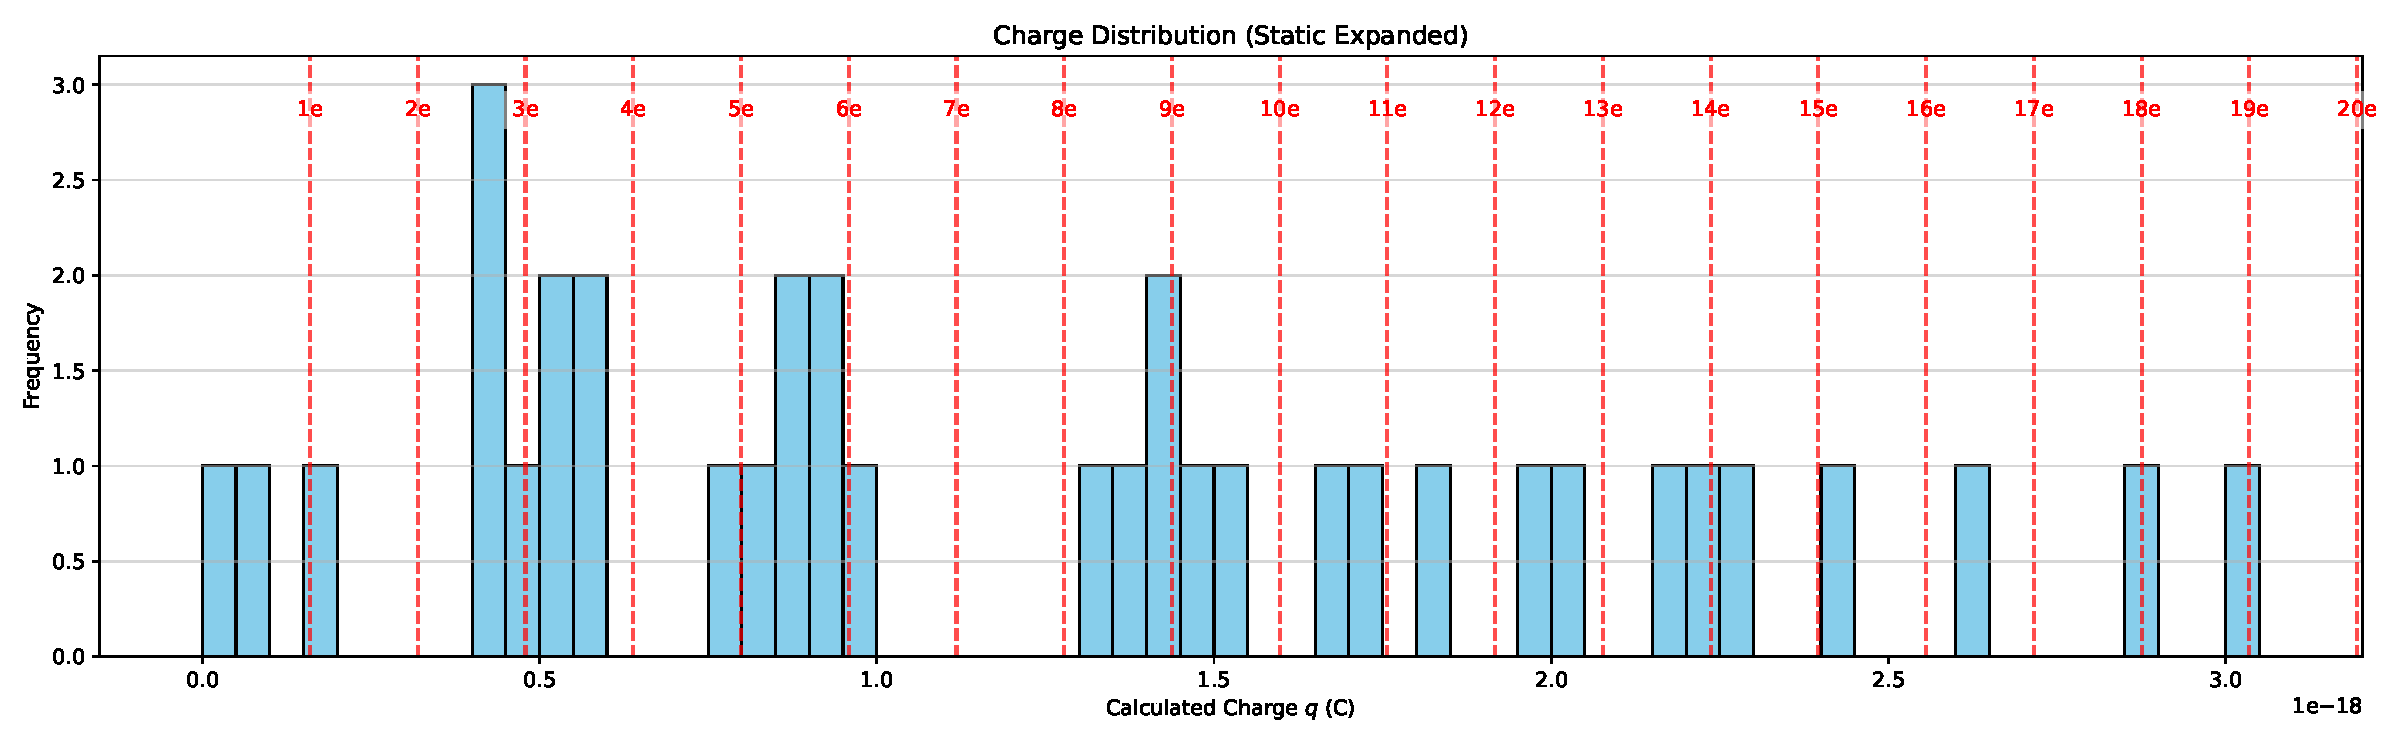
\includegraphics[width=0.98\linewidth]{plots/hist_static.pdf}\\
    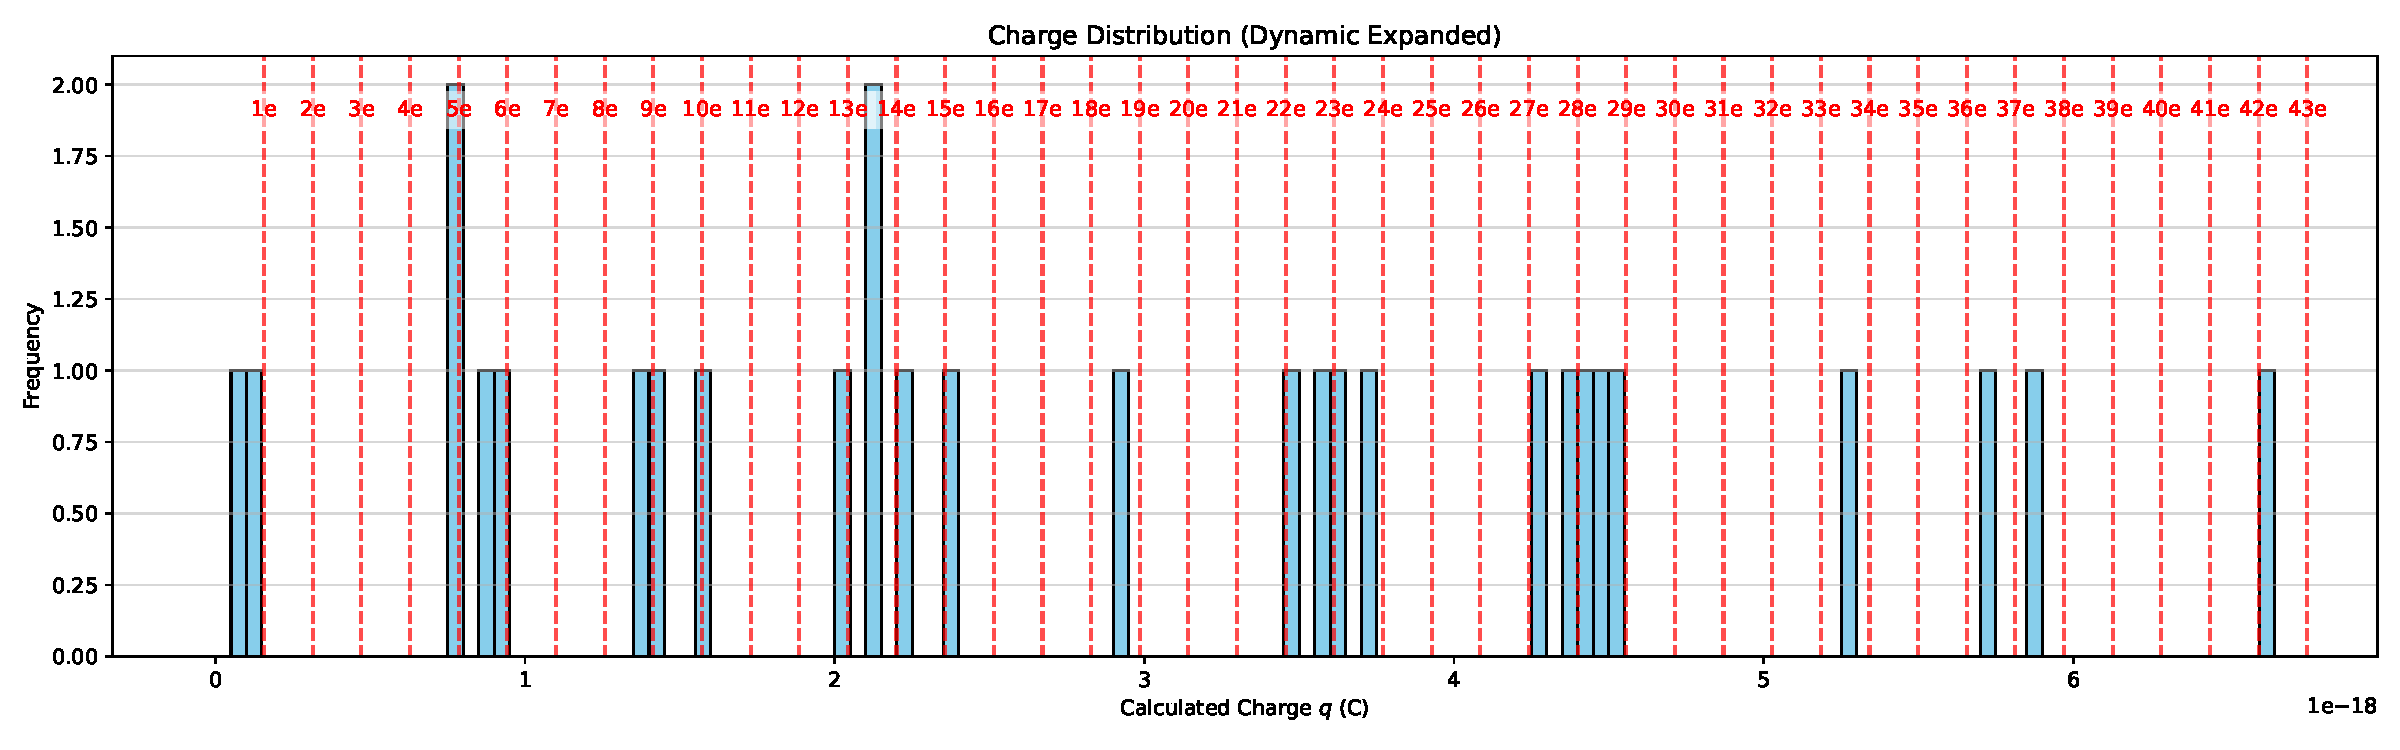
\includegraphics[width=0.98\linewidth]{plots/hist_dynamic.pdf}
    \caption{Histograms demonstrating the quantization of charge in the expanded Static and Dynamic datasets. The red dashed lines mark integer multiples of the experimentally derived elementary charge $e$.}
    \label{fig:histograms}
\end{figure}
\end{landscape}
% ------------------- Section 5: Post-Lab Questions -------------------
\section{Answers to Post-Lab Questions}

\subsection*{Q1: Calculate the average charge for both measurement methods.}
This has been achieved via the pairwise expansion and quantization search algorithm detailed in Section 4.3. The mean fundamental elementary charge $e$ derived from the Static Method is $1.597 \times 10^{-19}\text{ C}$, and from the Dynamic Method is $1.571 \times 10^{-19}\text{ C}$.

\subsection*{Q2: Mention the factors contributing to errors.}
Several physical and observational factors limit the precision of this experiment:
\begin{itemize}
    \item \textbf{Brownian Motion:} For extremely small droplets, random collisions with air molecules cause a jagged, non-linear path, skewing the timing over distance $S$.
    \item \textbf{Human Reaction Time:} Manually triggering a stopwatch introduces a reaction-time uncertainty ($\sim 0.1 - 0.2\text{ s}$), which becomes the dominant source of error for rapidly moving drops.
    \item \textbf{Convection Currents:} The intense illumination lamp heats the chamber, causing thermal air convection currents that impart unaccounted upward/downward forces on the droplet.
    \item \textbf{Evaporation / Shape:} If the oil evaporates or the droplet is not perfectly spherical, Stokes' law is violated, invalidating the derived equations.
\end{itemize}

\subsection*{Q3: Which of the two methods has less error. Why?}
The \textbf{Static Method} fundamentally has less error. This was empirically verified in our results ($0.29\%$ error for Static vs. $1.93\%$ for Dynamic). The reason is twofold:
First, the Static Method requires timing only one motion (the free fall $t$), whereas the Dynamic Method requires timing two separate motions ($t_1$ and $t_2$). This strictly doubles the human reaction time error. 
Second, finding a perfectly steady upward velocity $v_2$ in the Dynamic method is practically difficult due to slight non-uniformities in the capacitor's electric field and voltage fluctuations from the power supply.

\subsection*{Q4: Why shouldn't a drop be studied for a long time?}
A droplet suspended or moving in the chamber over a long period is subjected to two major hazards. Firstly, evaporation (or accumulation of condensation) changes the droplet's mass and radius, completely invalidating the previously measured $v_1$ parameter. Secondly, the droplet may randomly collide with stray background ions in the air (generated by cosmic rays or natural background radiation). This collision will discretely change its charge midway through observation, ruining the paired $v_1$ and $v_2$ measurements.

\subsection*{Q5: How do the drops become charged?}
The droplets primarily become charged via the \textbf{triboelectric effect} (friction). As the bulk oil is forcefully pushed through the narrow nozzle of the atomizer spray, friction between the fluid and the nozzle tears electrons away, leaving the resulting aerosolized mist droplets with a net positive or negative charge. In some advanced setups, a radioactive source or X-ray generator is specifically used to ionize the air and intentionally charge neutral drops.

\subsection*{Q6: By what other methods can the electric charge of an electron be measured?}
The elementary charge $e$ can be measured via several distinct macroscopic physical phenomena:
\begin{itemize}
    \item \textbf{Faraday's Laws of Electrolysis:} By measuring Faraday's constant $F$ (the charge of one mole of electrons) via electroplating, and utilizing Avogadro's number $N_A$, the charge is isolated: $e = F / N_A$.
    \item \textbf{Shot Noise in Vacuum Tubes:} Because electric current is composed of discrete charges, it is not perfectly smooth. By measuring the statistical variance (noise) of the current across a vacuum tube, Schottky's formula allows the calculation of $e$.
    \item \textbf{Quantum Hall Effect:} Using solid-state physics, the von Klitzing constant ($R_K = h/e^2$) and the Josephson constant ($K_J = 2e/h$) can be precisely measured. Solving this system yields an extraordinarily precise value for $e$.
\end{itemize}

\end{document}
